%%%%%%%%%%%%%%%%%%%%%%%%%%%%%%%%%%%%%%%%%
% Journal Article
% LaTeX Template
% Version 1.3 (9/9/13)
%
% This template has been downloaded from:
% http://www.LaTeXTemplates.com
%
% Original author:
% Frits Wenneker (http://www.howtotex.com)
%
% License:
% CC BY-NC-SA 3.0 (http://creativecommons.org/licenses/by-nc-sa/3.0/)
%
%%%%%%%%%%%%%%%%%%%%%%%%%%%%%%%%%%%%%%%%%

%----------------------------------------------------------------------------------------
%	PACKAGES AND OTHER DOCUMENT CONFIGURATIONS
%----------------------------------------------------------------------------------------

\documentclass[twoside]{article}

\usepackage{lipsum} % Package to generate dummy text throughout this template

\usepackage[sc]{mathpazo} % Use the Palatino font
\usepackage[T1]{fontenc} % Use 8-bit encoding that has 256 glyphs
\linespread{1.05} % Line spacing - Palatino needs more space between lines
\usepackage{microtype} % Slightly tweak font spacing for aesthetics

\usepackage[hmarginratio=1:1,top=32mm,columnsep=20pt]{geometry} % Document margins
%\usepackage{multicol} % Used for the two-column layout of the document
\usepackage[hang, small,labelfont=bf,up,textfont=it,up]{caption} % Custom captions under/above floats in tables or figures
\usepackage{booktabs} % Horizontal rules in tables
\usepackage{float} % Required for tables and figures in the multi-column environment - they need to be placed in specific locations with the [H] (e.g. \begin{table}[H])
\usepackage{hyperref} % For hyperlinks in the PDF

\usepackage{lettrine} % The lettrine is the first enlarged letter at the beginning of the text
\usepackage{paralist} % Used for the compactitem environment which makes bullet points with less space between them

\usepackage{abstract} % Allows abstract customization
\renewcommand{\abstractnamefont}{\normalfont\bfseries} % Set the "Abstract" text to bold
\renewcommand{\abstracttextfont}{\normalfont\small\itshape} % Set the abstract itself to small italic text

\usepackage{titlesec} % Allows customization of titles
%\renewcommand\thesection{\Roman{section}} % Roman numerals for the sections
%\renewcommand\thesubsection{\Roman{subsection}} % Roman numerals for subsections
%\titleformat{\section}[block]{\large\scshape\centering}{\thesection.}{1em}{} % Change the look of the section titles
%\titleformat{\subsection}[block]{\large}{\thesubsection.}{1em}{} % Change the look of the section titles

\usepackage{fancyhdr} % Headers and footers
\pagestyle{fancy} % All pages have headers and footers
\fancyhead{} % Blank out the default header
\fancyfoot{} % Blank out the default footer
%\fancyhead[C]{ April 2016 } % Custom header text
\fancyfoot[RO,LE]{\thepage} % Custom footer text

\usepackage[]{algorithm2e}
\usepackage{amsmath}
\usepackage{graphicx}
\graphicspath{ {images/} }
\usepackage{subfigure}
%----------------------------------------------------------------------------------------
%	TITLE SECTION
%----------------------------------------------------------------------------------------

\title{\vspace{-15mm}\fontsize{24pt}{10pt}\selectfont\textbf{Applying Classification Algorithms to Real-World Radio Pulse Data}} % Article title

\author{
\large
\textsc{Gene Der Su}\\
\normalsize University of California, Davis \\ % Your institution
\vspace{-5mm}
}
\date{}

%----------------------------------------------------------------------------------------

\begin{document}

\maketitle % Insert title

\thispagestyle{fancy} % All pages have headers and footers

%----------------------------------------------------------------------------------------
%	ABSTRACT
%----------------------------------------------------------------------------------------

\begin{abstract}

%\noindent \lipsum[1] % Dummy abstract text
\noindent The Quail Ridge Automated Animal Tracking (QRAAT) system performs inaccurate position calculations due to the noise received in the radio receivers. In order to increase the accuracy, the system needs a method to distinguish a noise event from a true radio pulse event before applying the position calculation. Using the nine variables collected by the receiver and millions of examples of training data, one can develop a classification algorithm to determine whether an observation is a pulse event or a noise event. The training data is labeled with two different techniques. One of the techniques, Likelihood Labeling, labels the observation with a high likelihood in the expected direction as pulse and the rest as noise. Another technique, Manual Labeling, labels the observation that visually looks correct as pulse and the rest as noise. The methods implemented to classify the data are Bayes Classifier, Random Forests, and Support Vector Machine. The evaluation is done with the 10-fold cross-validation to determine which method is the best to use in the QRAAT system. We found that the Random Forests algorithm produced the best classification.

\end{abstract}

%----------------------------------------------------------------------------------------
%	ARTICLE CONTENTS
%----------------------------------------------------------------------------------------

%\begin{multicols}{2} % Two-column layout throughout the main article text

\section{Introduction}

%\lettrine[nindent=0em,lines=3]{L} orem ipsum dolor sit amet, consectetur adipiscing elit.
%\lipsum[2-3] % Dummy text
\subsection{Background}
The Quail Ridge Automated Animal Tracking (QRAAT) system provides ecological researchers with tracking data from small wild animals such as birds and rodents. This system consists of transmitters, a number of radio receiver towers, and a central processing server. Transmitters, which transmit radio pulses, are attached to each animal. The receiver towers, which receive the radio pulses, are stationary and located throughout the Quail Ridge Reserve. The receiver towers send the received data to the central processing server. The central processing server then uses the data collected from each of the receiver towers to calculate the most likely position of the animal. 

In addition, each of the radio receiver towers has a detector that captures the signal of interest. The receiver towers continuously receive radio data from the surroundings. The detector computes the sum of the signal amplitude within a time window. If this sum passes an amplitude threshold, then it is considered a signal of interest and will be used in the position calculation. However, there are other sources such as car engines that create high amplitude radio pulses. The detector is unable to distinguish these from a true pulse event. There is also low-level random background noise being collected with the signal of interest. The latter is not much of a problem, but distinguishing true pulse events from high-amplitude noise is difficult.  

Due to the carrying capacity of small animals, the batteries of the transmitters are generally small. The researchers have to reduce the signal strength in exchange for a longer battery life. The pulse with the reduced signal strength becomes even more difficult to distinguish from the noise. Hence the resulting positions can be significantly far away from the targeted animals. The QRAAT system needs a more sophisticated algorithm to differentiate the pulse from the noise before preforming the position calculation.



\subsection{Problem Description}
For every high-amplitude event, the radio receivers collect nine variables. Band3 is the bandwidth at power 3dB. Band10 is the bandwidth at power 10dB. Frequency is the frequency of the signal. EC is the confidence of eigenvalue decomposition. TNP is the total noise power of the signal. EDSP is the eigenvalue decomposition signal power. FDSP is the Fourier decomposition signal power. EDSNR is the eigenvalue decomposition signal to noise ratio which is proportional to EDSP/TNP. FDSNR is the Fourier decomposition signal to noise ratio which is proportional to FDSP/TNP. We used a total of 7,151,826 unlabeled observations in this project. The goal of the project is to use these datasets to develop a classification algorithm that will be the most suitable for the QRAAT system. 

\subsection{Datasets}
The data is organized by different combinations of deployment and site . A single deployment refers to a specific transmitter on an animal for tracking while a single site refers to a specific radio receiver tower for collecting data. Different combinations of deployment and site are expected to exhibit different behaviors of the same variables and are therefore treated as separate datasets. 

\begin{compactitem}
\item Deployment 57 is a stationary wood rat transmitter (low signal strength transmitter) with a known location. The timestamp (seconds from Unix epoch) is from 1382252400 to 1385366400 (10/20/2013 - 11/25/2013). There are a total of 2,222,486 observations. Site 2 has 649,060 observations. Site 3 has 881,529 observations. Site 5 has 363,391 observations. Site 6 has 328,506 observations.
\item Deployment 60 is a stationary beacon (high signal strength transmitter) with a known location. The timestamp  (seconds from Unix epoch) is from 1383012615 to 1384222215 (10/28/2013 - 11/11/2013). There are a total of 4,874,724 observations. Site 1 has 1,224,901 observations. Site 2 has 656,838 observations. Site 3 has 762,951 observations. Site 4 has 655,953 observations. Site 5 has 398,872 observations. Site 6 has 721,619 observations. Site 8 has 453,590 observations.
\item Deployment 61 and 62 are two different moving wood rat transmitters with GPS tracking. Two transmitters moved together during two periods of trackings. The first tracking is from timestamp  (seconds from Unix epoch) 1391276584 to 1391285374 (2/1/2014, 9:43am to 12:09pm). Deployment 61 has 11,191 total observations, deployment 62 has 22,422 total observations, and the tracking has 8,388 gps observations. 
\item Second tracking of deployment 61 and 62 are from timestamp  (seconds from Unix epoch) 1396725597 to 1396732326 (4/5/2014, 12:19pm to 2:12pm). Deployment 61 has 11,672 total observations, deployment 62 has 9,331 total observations, and the tracking has 6,438 gps observations.

\end{compactitem}

\subsection{Labeling}
There are two techniques to label the data. One technique is to use the GPS location to determine the label of the observation. Another technique is to use the visual recognition of the human eye to detect patterns in the data that are clearly either noise or pulse.
\subsubsection{Likelihood Labeling}
The position calculation is the linear combination of the likelihoods of the data collected during a period of time. The position with the highest likelihood is chosen to be the estimate of the location of the animal. For each observation, the system can determine the likelihood of a specific angle of the transmission's origin. Given the likelihood of the bearing, the direct way to label an observation is by using a threshold on the likelihood at the angle given by the GPS. The observations with high likelihood from the direction of the GPS records are marked as pulses while the ones with low likelihood are marked as noise (see figure 1). The drawback of this method is that the likelihood threshold seems to be inconsistent between different combinations of deployment and site based on a visual inspection (see figure 2). Some combinations of deployment and site require lower threshold to separate the pulse and the noise while others read higher threshold. One can only choose a threshold to define the good observations. The likelihood threshold chosen to label this data is 0.7.
\begin{figure}[h]
\centering
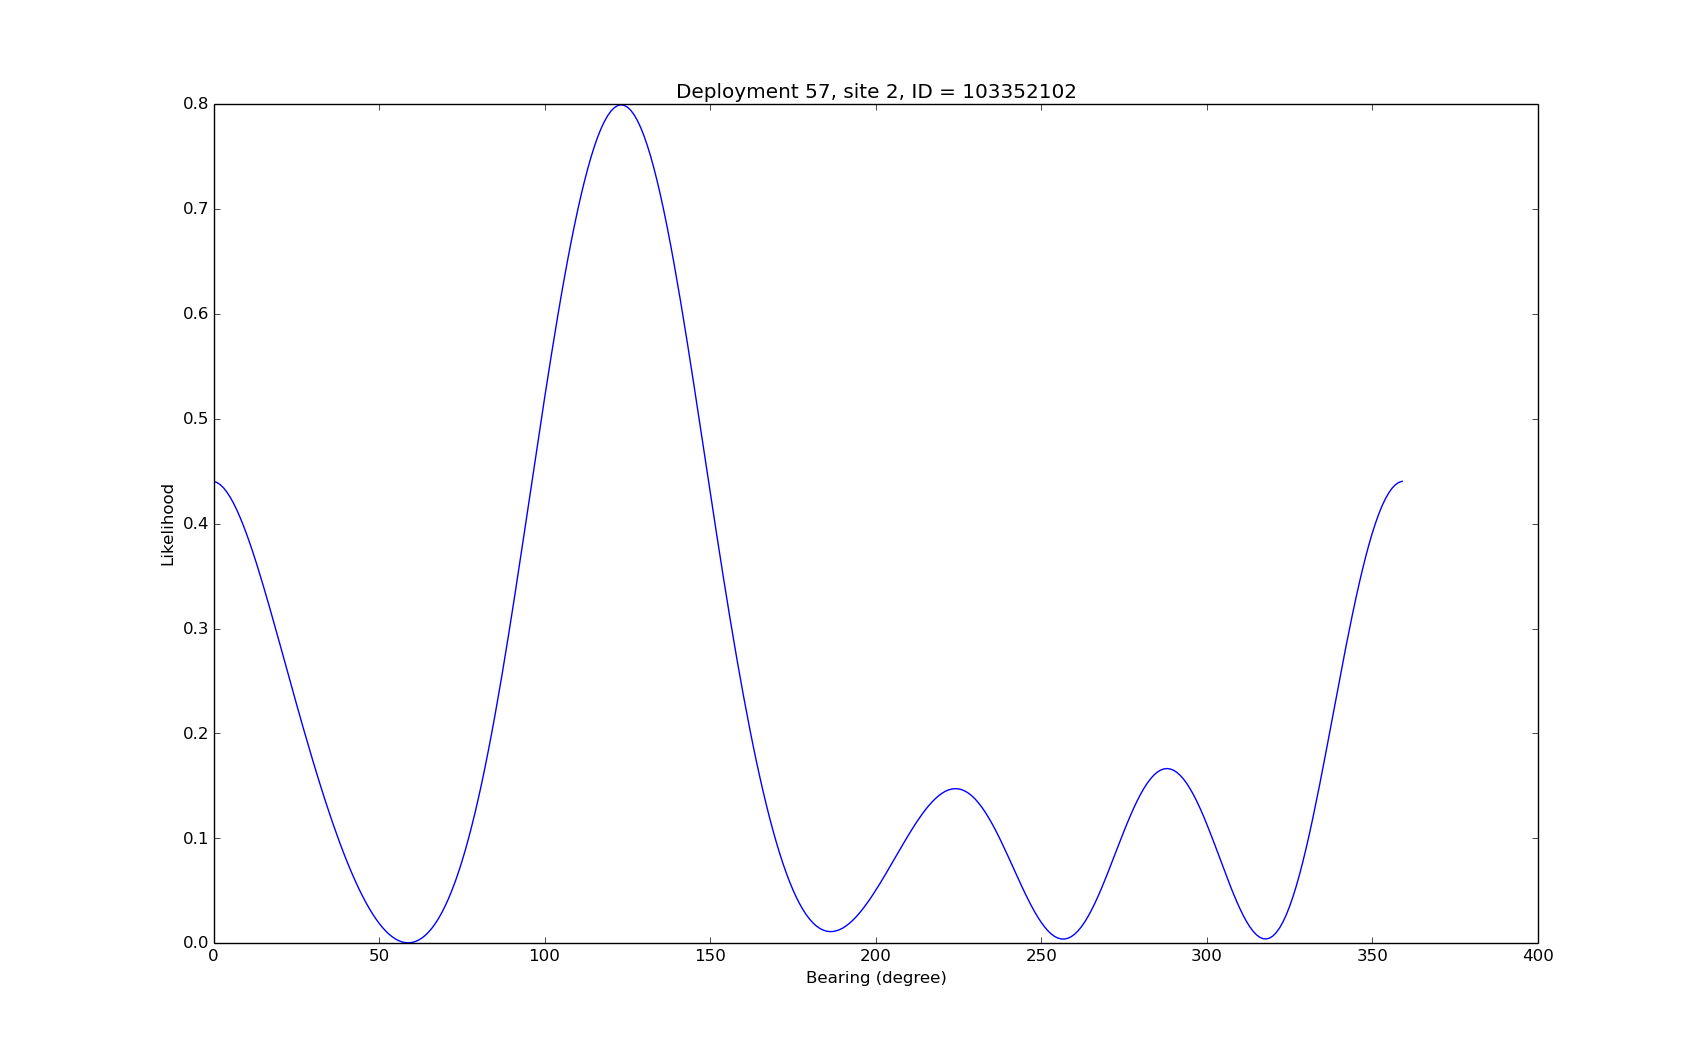
\includegraphics[width=\textwidth]{bearingPlot}
\caption{A plot of bearing likelihood for an observation. There are four local maxima each near 0, 125, 225, and 290 degree. The expected angle for deployment 57 at site 2 is 124.15 degree which indicates that this is a good observation. This observation will give the expected angle (124.15 degree) the most weight (0.8) in the position calculation while giving other angles much lower weights.}
\end{figure}

\begin{figure}[ht!]
     \begin{center}
%
        \subfigure[Deployment57, Site 2]{%
            \label{fig:first}
            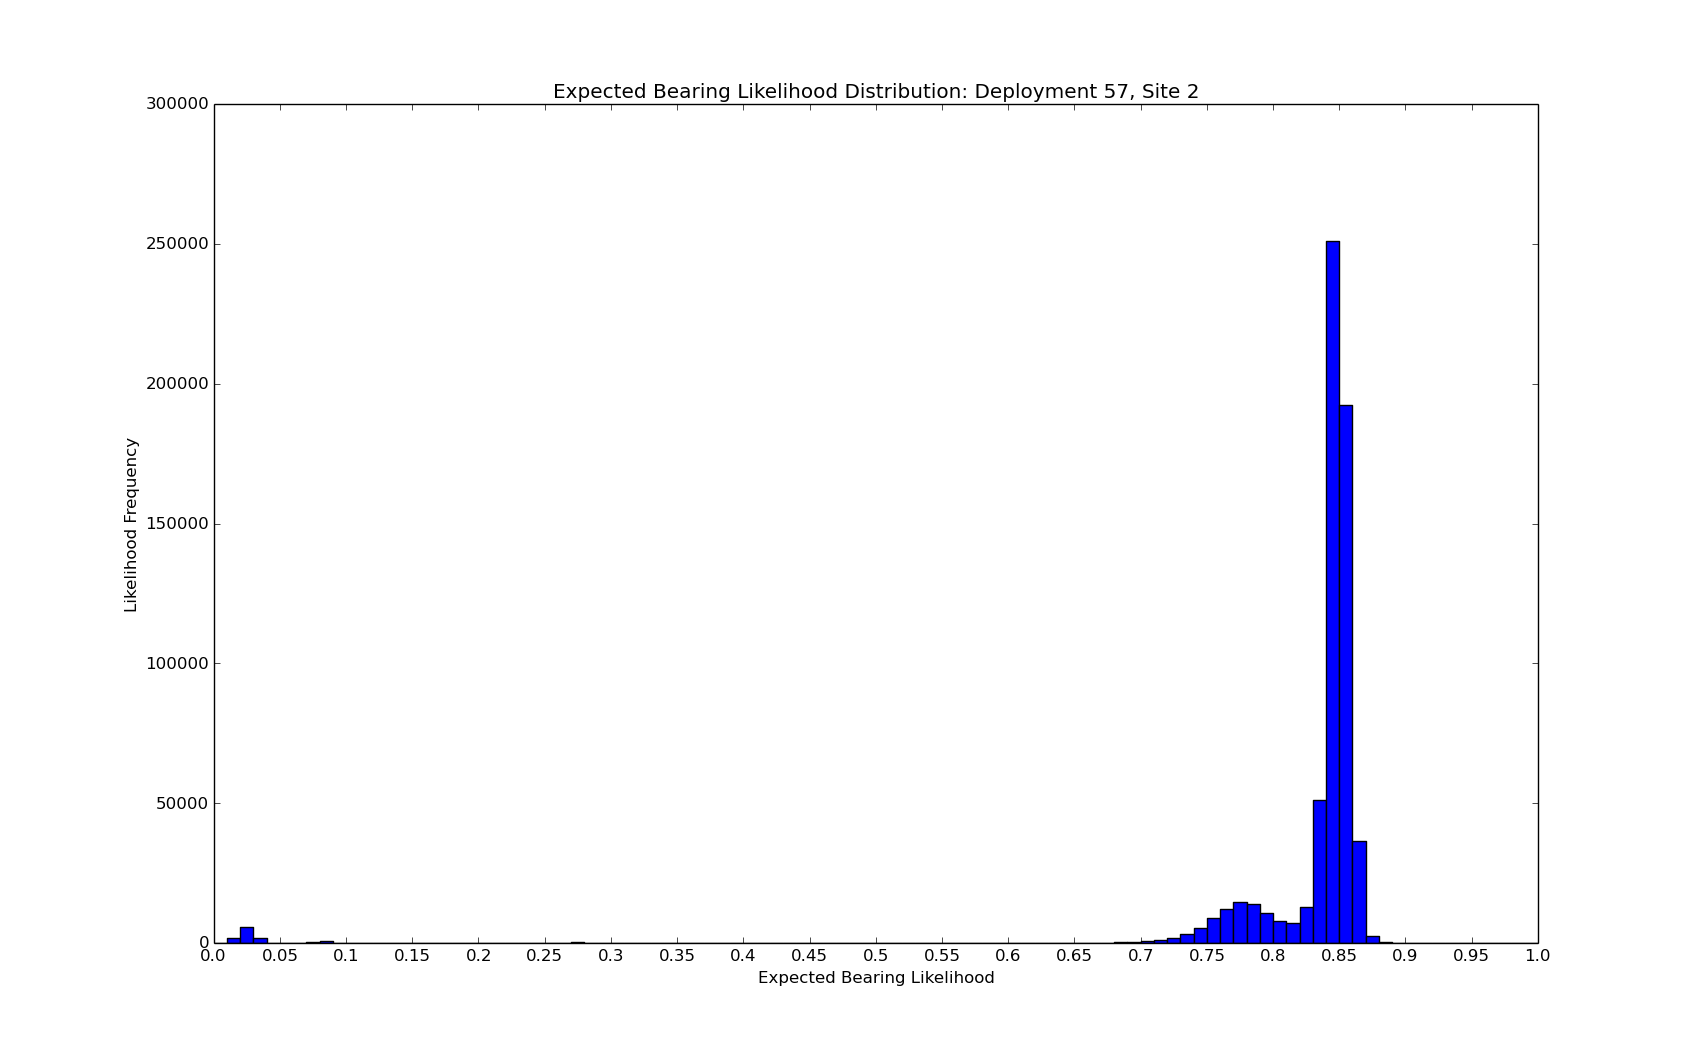
\includegraphics[width=0.5\textwidth]{Deployment57_site2}
        }%
        \subfigure[Deployment57, Site 3]{%
           \label{fig:second}
           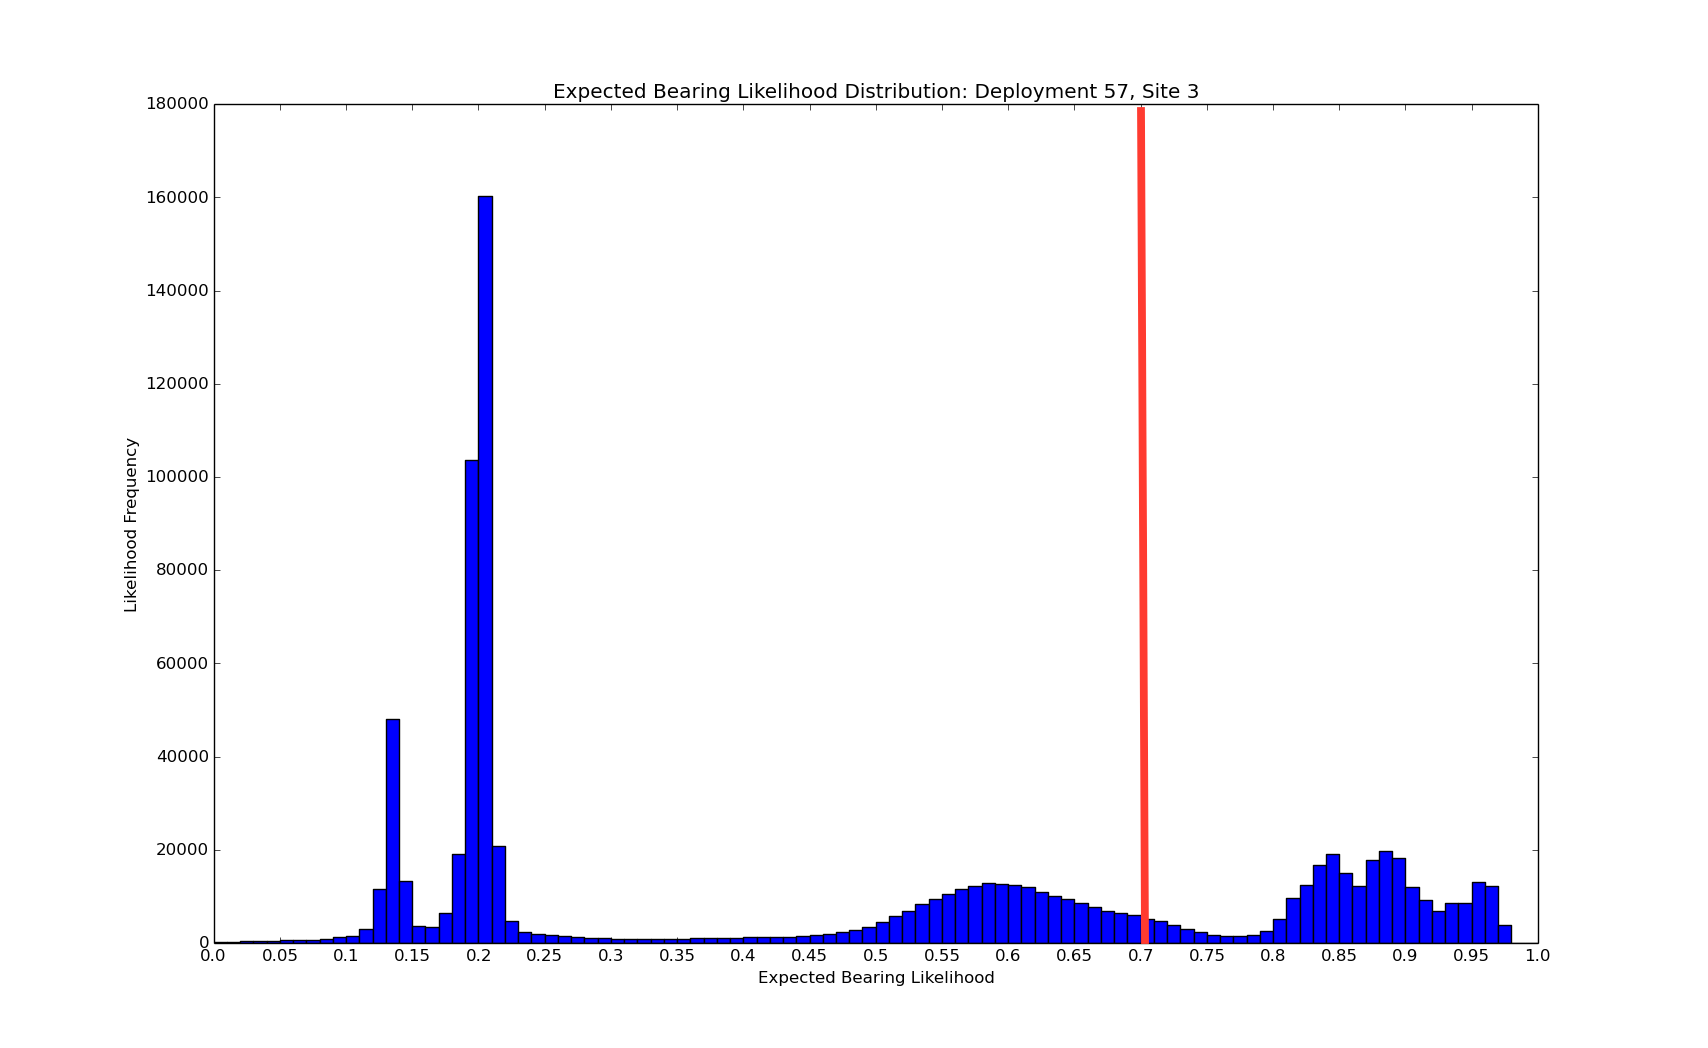
\includegraphics[width=0.5\textwidth]{Deployment57_site3}
        }\\ %  ------- End of the first row ----------------------%
        \subfigure[Deployment57, Site 5]{%
            \label{fig:third}
            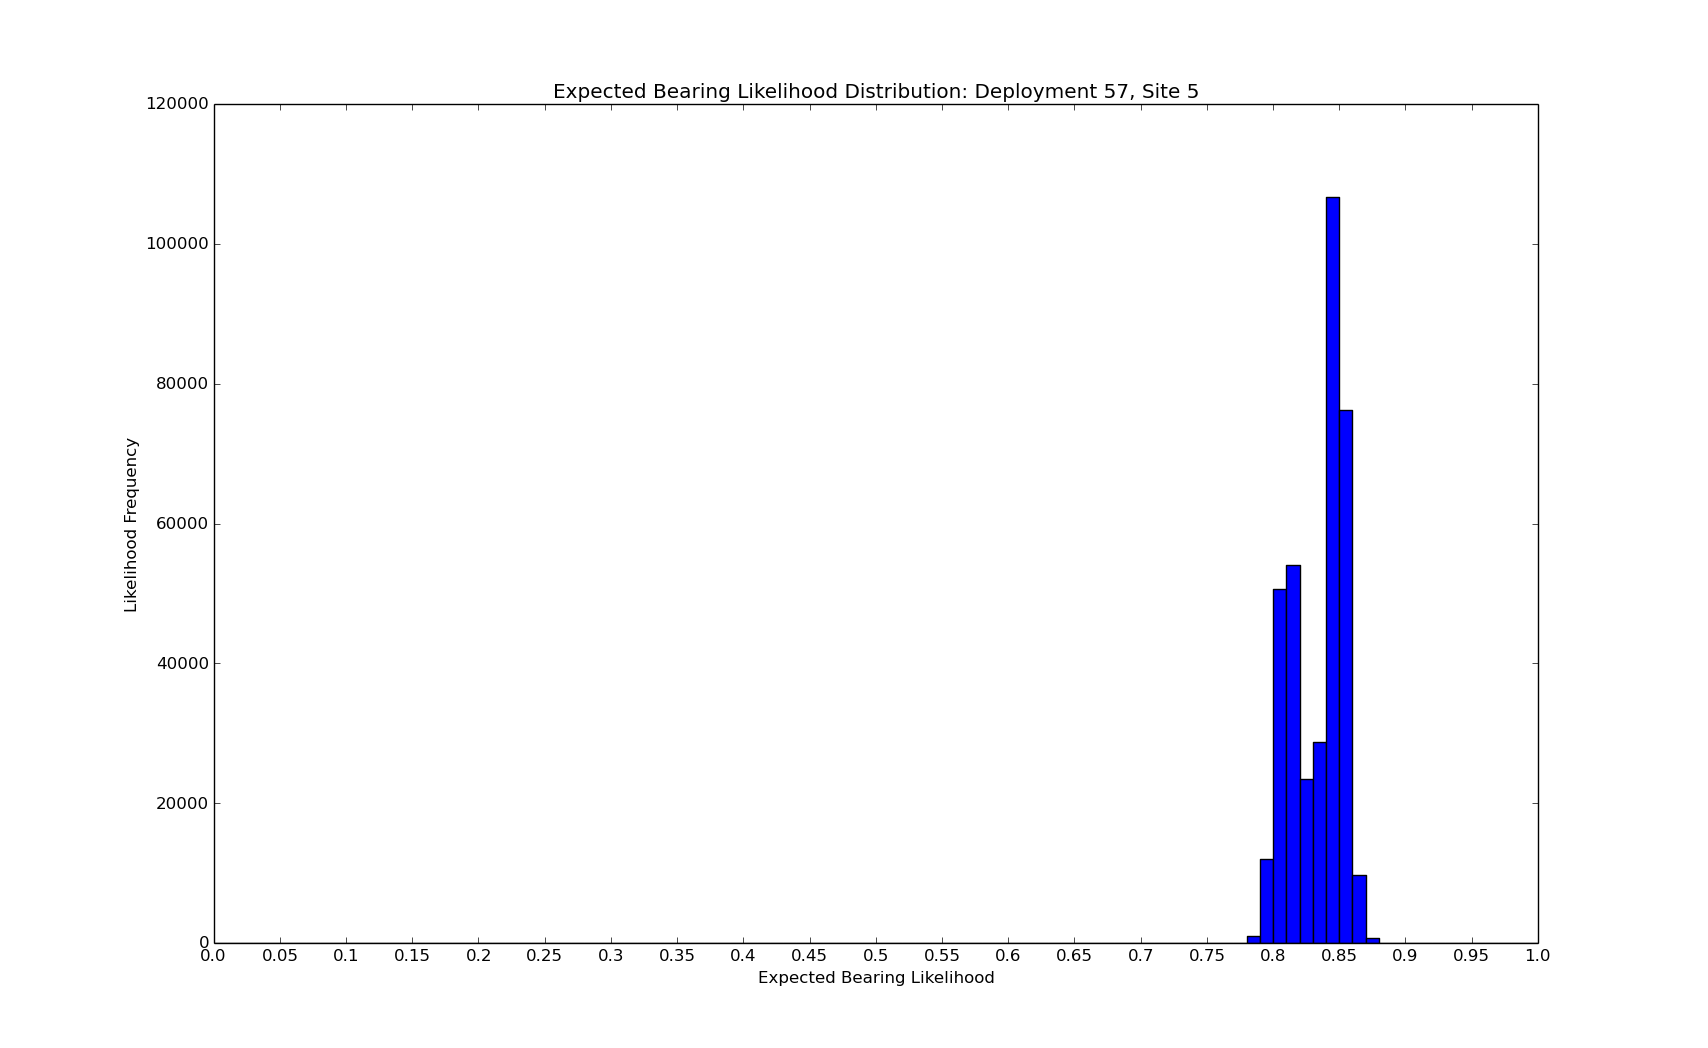
\includegraphics[width=0.5\textwidth]{Deployment57_site5}
        }%
        \subfigure[Deployment57, Site 6]{%
            \label{fig:fourth}
            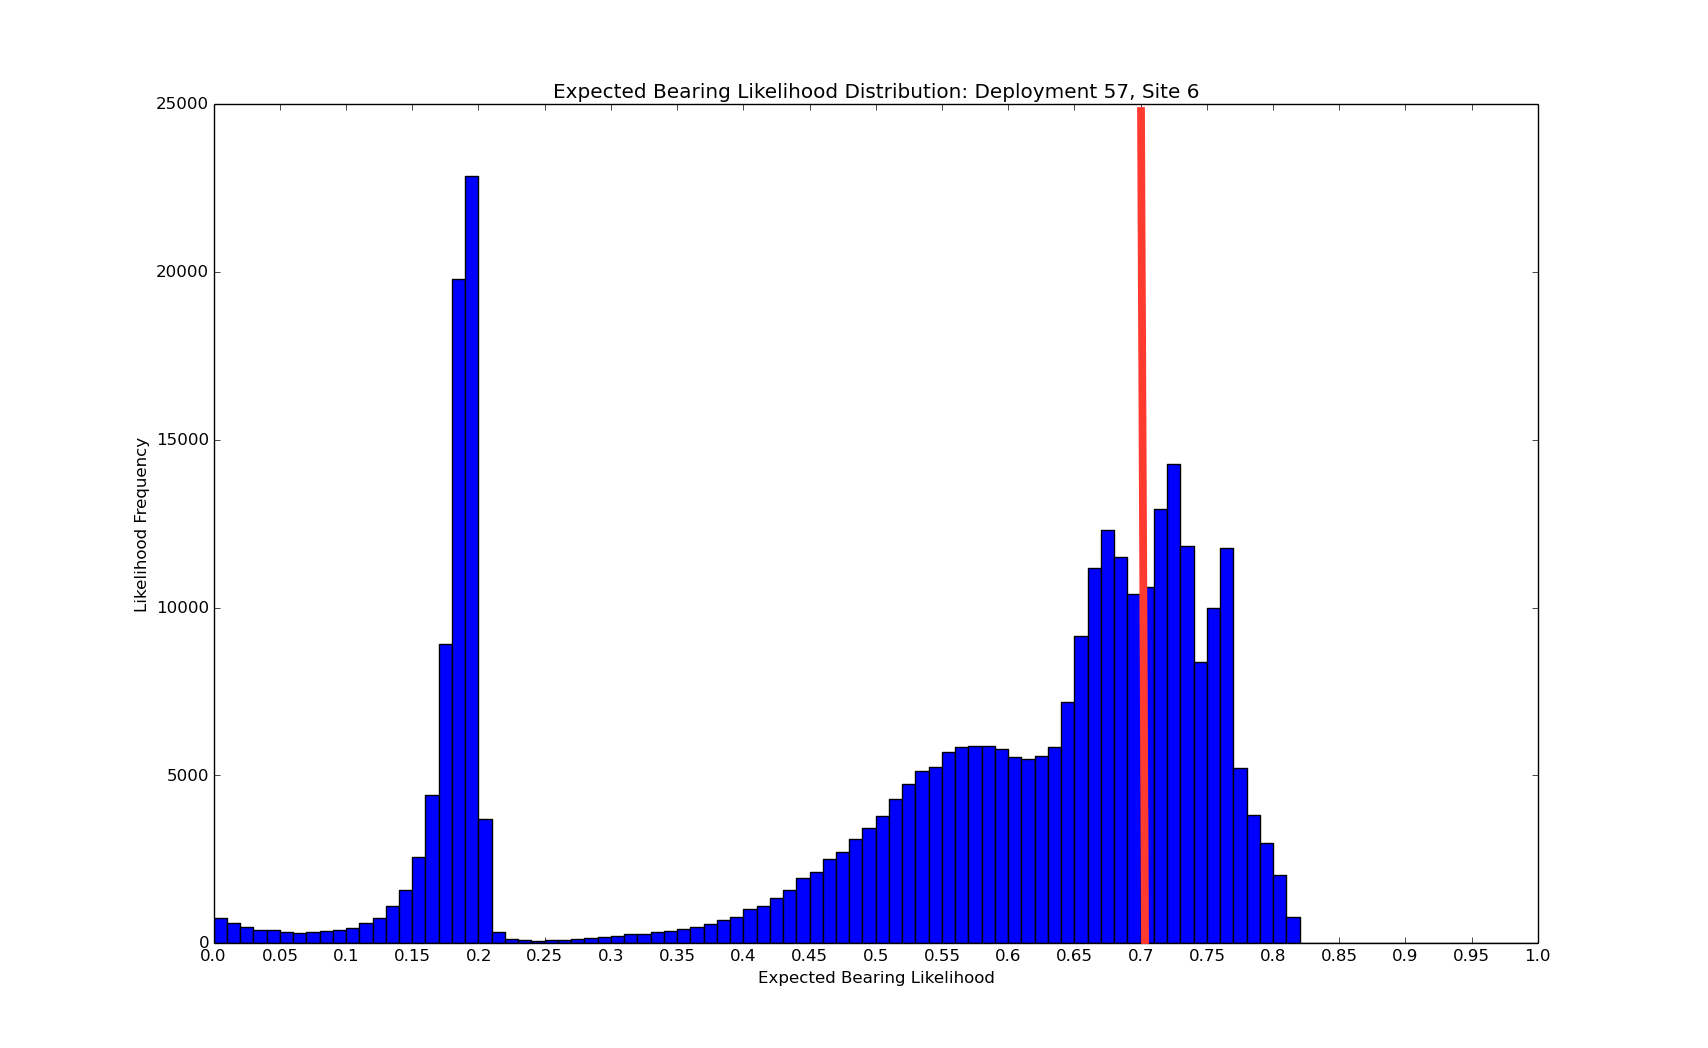
\includegraphics[width=0.5\textwidth]{Deployment57_site6}
        }%
%
    \end{center}
    \caption{%
       The plots are expected bearing likelihood and its frequency distributions for each site used for deployment 57.  The x-axis represents the likelihood of the observation at the GPS location. The y-axis represents the frequency of the likelihood. Different sites showed different distributions of the likelihood measures. Site 2 and site 5 got much of good pulses with very little noises while site 3 and site 6 has little pulses and wide distributions of noises. A threshold of 0.7 (marked as the red line) at the expected bearing is chosen to be the definition of a good observation in the likelihood labeling.
     }%
   \label{fig:subfigures}
\end{figure}

\subsubsection{Manual Labeling}
When the signal strength is high, the pulse can be easily distinguished visually from the noise by plotting the data. From the plotted data, there are patterns to determine whether an observation is pulse or noise (see figure 3). The strategy is to plot each of the nine variables versus time and set a threshold to separate the pulse and the noise. The disadvantage of this technique is that one has to manually go through each combination of deployment, site, and variable to determine the thresholds. This process is not only time consuming but may include bias toward the labeling. 

\begin{figure}[ht!]
     \begin{center}
%
        \subfigure[Time VS Band3]{%
            \label{fig:first}
            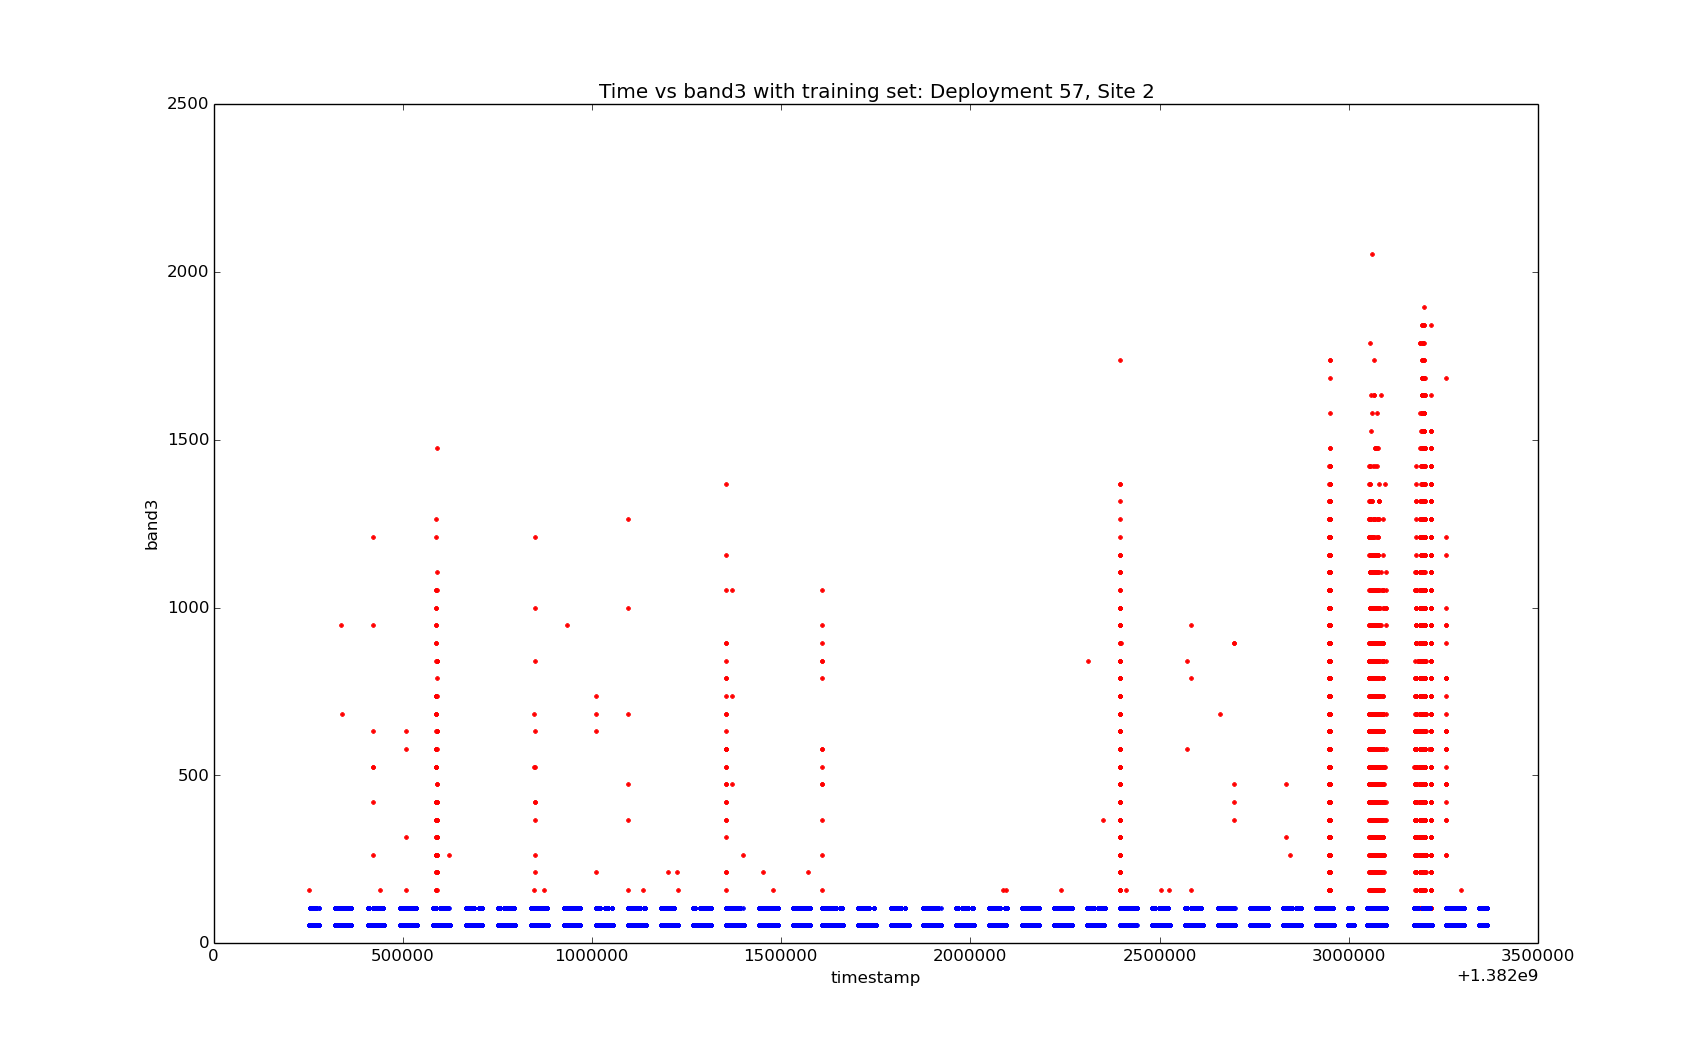
\includegraphics[width=0.5\textwidth]{Deployment57_band3_site2}
        }%
        \subfigure[Time VS Frequency]{%
           \label{fig:second}
           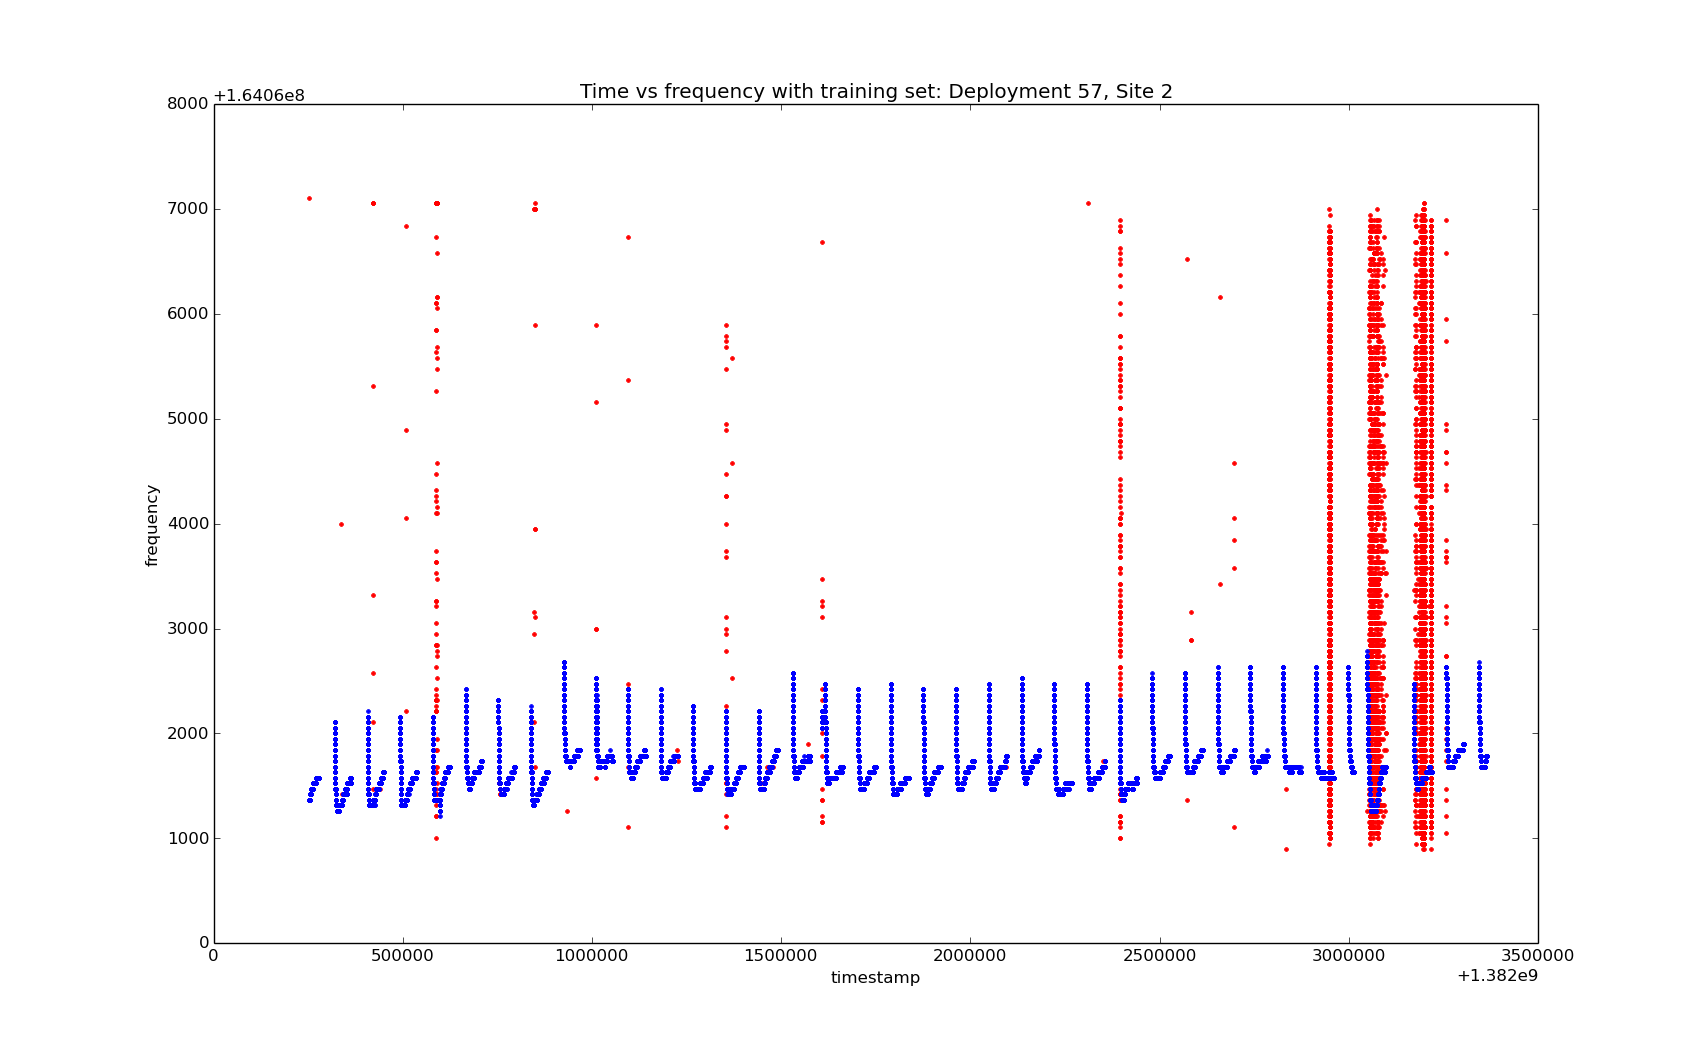
\includegraphics[width=0.5\textwidth]{Deployment57_frequency_site2}
        }
    \end{center}
    \caption{%
        The plot shows labeling results for manual labeling with red as noise and blue as pulse. The manual labeling manually go through each combinations of deployment, site, and variable and determine the best thresholds on each combination to visually separate noise from pulse. 
     }%
   \label{fig:subfigures}
\end{figure}

\hfill \break
\noindent
Both Likelihood Labeling and Manual Labeling have their advantages and disadvantages. Since one technique is not better than the other, both techniques will be used in the evaluation independently.


%------------------------------------------------

\section{Methods}
There are three classification algorithms described in this section: Naive Bayes Classifier, Random Forests, and Support Vector Machine. Each of them have their advantages and disadvantages. This section will go through the implementation of each method in detail and troubleshoot some issues working on out real-world data. The pseudocode for each method are also described after each subsection. The results will be described in the evaluation section.

\subsection{Naive Bayes Classifier}
Naive Bayes Classifier is one of the simplest classifiers that one can implement. It uses Bayes' Theorem to calculate the probability of a class given an observation while assuming all variables are independent. Provided a training set, one must first determine the probability distribution of each variable given a class. All variables are assumed to be normally distributed. Hence the mean and the variance of each variable given a class are calculated and stored in the database. During the process of classification, one can determine the probability of each class given the data by Bayes' Theorem. The class with the highest probability will determine the class of the observation.

\begin{align*}
\text{Bayes Theorem (with 9 varia}&\text{bles and variable independenance assumption):}\\
p(class_i | x) &= \frac{p(class_i) \prod\limits_{j=1}^{9}  p(x_j|class_i)}{p(x)}\\
&\propto p(class_i) \prod\limits_{j=1}^{9}  p(x_j|class_i)
\end{align*}

Since the denominator of the probability is constant throughout the calculation of the probability of each class, only the numerator of the probability will be considered. It is important to note that all the probabilities are small numbers, thus, repeatedly multiply the probabilities from each variable will result in a loss of floating point precision. A common way to fix this problem is to use the log probability (likelihood) instead of the original probability. By taking the log of Bayes' Theorem, the likelihood of a class becomes the sum of the log probability of the individual variable. Moreover, the exponential function can be removed when applied log probability if the distribution is assumed to be Gaussian.

\begin{align*}
\text{Log probability:}\\
log(p(class_i | x)) &\propto log(p(class_i)) + \sum\limits_{j=1}^{9}  log(p(x_j|class_i)) \\
&= log(p(class_i)) - \sum\limits_{j=1}^{9}  ( \frac{(x_j - \mu_{class_i})^2}{2\sigma_{class_i}^2} + 0.5log(2\pi\sigma_{class_i}^2))
\end{align*}

Although the assumption of all variables being normally distributed works well on continuous variables, discrete variables should be treated more carefully. In the QRAAT system, band3, band10, and frequency are collected as discrete variables with a few high-occurrence values. These three variables should be treated as a mixed probability distribution where the high occurrence values each have a unique probability while other values are treated as Gaussian to insure the possibility of nonzero probabilities. We store the proportions of these unique values and normalize the overall mixed probability to 1 during the training process. 

\IncMargin{1em}
\begin{algorithm}
\SetKwData{Left}{left}\SetKwData{This}{this}\SetKwData{Up}{up}
\SetKwFunction{Union}{Union}\SetKwFunction{FindCompress}{FindCompress}
\SetKwInOut{Input}{input}\SetKwInOut{Output}{output}
\Input{A labeled training set, $P$ for data labeled as pulse and $N$ for data labeled as noise}
\Output{Mean and variance of data stored in database}
\BlankLine
\For{i in each data type}{
\tcp{if i is discrete, remember to consider mixed probability}
\emph{calculate mean and variance of P}\;
\emph{store mean and variance in the database with pulse class and i data type}\;
\emph{calculate mean and variance of N}\;
\emph{store mean and variance in the database with noise class and i data type}\;
}
\caption{Naive Bayes Classifier trainer}\label{NBCt}
\end{algorithm}\DecMargin{1em}

\IncMargin{1em}
\begin{algorithm}
\SetKwData{Left}{left}\SetKwData{This}{this}\SetKwData{Up}{up}
\SetKwFunction{Union}{Union}\SetKwFunction{FindCompress}{FindCompress}
\SetKwInOut{Input}{input}\SetKwInOut{Output}{output}
\Input{An observation X with unknown class}
\Output{Class determined by the model}
\BlankLine
\emph{set likelihood\_P = 0 and likelihood\_N = 0}\;
\For{i in each data type}{
\emph{likelihood\_P += log probability of P given X\_i}\;
\emph{likelihood\_N += log probability of N given X\_i}\;
}
\uIf{likelihood\_P > likelihood\_N}{\emph{return P}\;}
\Else{\emph{return N}\;}
\caption{Naive Bayes Classifier}\label{NBC}
\end{algorithm}\DecMargin{1em}


\subsection{Random Forests}
Random Forests is a method that uses a collection of Decision Trees to classify data. A Decision Tree is simple to visualize (see figure 4). It uses a tree as a structure to decide into which class an observation should be classified. When given a decision tree and an observation, one can traverse the tree according to the constraints at each node and determine the class at the leaf node. However, when trained on different subsets of the data, the Decision Trees will have great variations. To remove the effect of this data dependance, one can create multiple trees using different bootstrapped data and use a majority vote of these trees for classification. If there's a strong predictor variable, each of decision trees will have high chance of using this variable, causing the trees to be correlated. To remove this effect, one can pick a subset of allowable variables at each split. The random forests algorithm builds a specific amount of trees and use the majority vote as the result of the classification. Each tree is built using N bootstrapped observations from the training set where N is the number of training set observations. Given this set, the algorithm will subsampling m variables at each split where the number of variables used, m, is typically $\sqrt{p}$ where p is the number of variables in the data. It finds the best split by calculating entropies at each point of each m variables. The split with the lowest weighted sum of entropy for the child nodes will be used to create the node. The child nodes then call the algorithm recursively until one of the terminating conditions is met. 
\\\\The terminating conditions are:
\begin{itemize}
\item the number of observations being less than 2
\item all records has the same class
\item all records has the same variable values
\end{itemize}
If the child terminates, a leaf node will be attached with the highest occurrence class for classification in that leaf. Three variables at each split and nine trees to classify is chosen to train the QRAAT datasets.

\begin{align*}
weightedEntropy(child_{left}, child_{right}) =& \frac{|child_{left}|}{|child_{left}| + |child_{right}|}(- \frac{|child_{left_{pulse}}|}{|child_{left}|}log(\frac{|child_{left_{pulse}}|}{|child_{left}|}) \\
&- \frac{|child_{left_{noise}}|}{|child_{left}|}log(\frac{|child_{left_{noise}}|}{|child_{left}|}))\\
&+\frac{|child_{right}|}{|child_{left}| + |child_{right}|}(- \frac{|child_{right_{pulse}}|}{|child_{right}|}log(\frac{|child_{right_{pulse}}|}{|child_{right}|}) \\
&- \frac{|child_{right_{noise}}|}{|child_{right}|}log(\frac{|child_{right_{noise}}|}{|child_{right}|}))\\
\end{align*}

\begin{figure}[h]
\centering
\includegraphics[width=\textwidth]{DecisionTree}
\caption{A small sample of the decision tree trained with deployment 60, site 3, likelihood labeling data. The original tree contains 9659 nodes, hence only a small portion is shown in the figure.}
\end{figure}

\IncMargin{1em}
\begin{algorithm}
\SetKwData{Left}{left}\SetKwData{This}{this}\SetKwData{Up}{up}
\SetKwFunction{Union}{Union}\SetKwFunction{FindCompress}{FindCompress}
\SetKwInOut{Input}{input}\SetKwInOut{Output}{output}
\Input{A labeled training set, $S$. Decision Tree, $T$.}
\Output{Decision Tree}
\BlankLine
\tcp{finding the best variable and value to split the data}
\emph{set bestEntropy = 1, bestDataType = -1, and bestSplitValue = -1}\;
\emph{dataType = random sample of 3 variables}\;
\For{i in dataType}{
\uIf{|S| > 100}{
\For{j in each 100 intervals between min and max}{
\emph{calculate weighted entropy at split(S\_i[j])}\;
\If{entropy < bestEntropy}{
\emph{bestEntropy = entropy, bestDataType = i, bestSplitValue = S\_i[j]}\;
}}}
\Else{
\For{j in each S\_i}{
\emph{calculate weighted entropy at split(S\_i[j])}\;
\If{entropy < bestEntropy}{
\emph{bestEntropy = entropy, bestDataType = i, bestSplitValue = S\_i[j]}\;
}}}}
\emph{split data into SL and SR according to the bestDataType and bestSplitValue}\;
\emph{create a branch node in the tree with bestDataType and bestSplitValue}\;
\tcp{check for termination and recursive calls}
\uIf{|SL| <= 1 or all SL has same class or all SL has same variables}{
\emph{create a leaf node in the tree with the class with most occurrence}\;}
\Else{\emph{recursive call with SL as training set and the current tree as the decision tree}\;}
\uIf{|SR| <= 1 or all SR has same class or all SR has same variables}{
\emph{create a leaf node in the tree with the class with most occurrence}\;}
\Else{\emph{recursive call with SR as training set and the current tree as the decision tree}\;}
\caption{Decision Tree building}\label{DCb}
\end{algorithm}\DecMargin{1em}

\IncMargin{1em}
\begin{algorithm}
\SetKwData{Left}{left}\SetKwData{This}{this}\SetKwData{Up}{up}
\SetKwFunction{Union}{Union}\SetKwFunction{FindCompress}{FindCompress}
\SetKwInOut{Input}{input}\SetKwInOut{Output}{output}
\Input{A labeled training set, $S$.}
\Output{Resulting forests}
\BlankLine
\emph{set forests = empty array}\;
\For{i from 0 to 9}{
\emph{B = Bootstrap |S| samples from S}\;
\emph{T\_i = tree built with Decision Tree Building (Algorithm 3) and dataset B}\;
\emph{forests append T\_i}\;
}
\caption{Random Forests trainer}\label{RFt}
\end{algorithm}\DecMargin{1em}

\IncMargin{1em}
\begin{algorithm}
\SetKwData{Left}{left}\SetKwData{This}{this}\SetKwData{Up}{up}
\SetKwFunction{Union}{Union}\SetKwFunction{FindCompress}{FindCompress}
\SetKwInOut{Input}{input}\SetKwInOut{Output}{output}
\Input{An observation $X$ with unknown class}
\Output{Class determined by the model}
\BlankLine
\emph{set class\_P = 0 and class\_N = 0}\;
\For{i from 0 to 9}{
\emph{class = class determined by traverse forests[i]}\;
\uIf{class == P}{\emph{class\_P += 1}\;}
\Else{\emph{class\_N += 1}\;}
}
\uIf{class\_P > class\_N}{\emph{return P}\;}
\Else{\emph{return N}\;}
\caption{Random Forests classifier}\label{RFc}
\end{algorithm}\DecMargin{1em}

\subsection{Support Vector Machine}
A Support Vector Machine (SVM) is a method that uses a hyperplane to separate two classes. The shape of the hyperplane is governed by the choice of kernel. A simple choice of $K(x,x') = x \cdot x'$ will result a linear boundary as the hyperplane where as $K(x,x') = (1 + x \cdot x')^n$ will result a n-degree polynomial boundary. Other popular choice of kernels are Gaussian radial basis function $K(x,x') = exp(-\gamma |x - x'|^2)$ and hyperbolic tangent $K(x,x') = tanh(\kappa x \cdot x' + c)$. By replacing the equation with a different kernel, SVM can efficiently classify data with different spatial mappings. The Gaussian radial basis function is chosen to be used in this project because of its property of separating a cluster of data. The hyperplane is then calculated by finding the Lagrange multipliers that maximize the Lagrangian dual problem subject to the constraints and the KKT conditions. The simplest way to solve this optimization problem is using Platt's sequential minimal optimization (SMO). The algorithm tries to optimize two multipliers at a time while setting all other variables constant. When optimizing two variables with the conditions, such optimization becomes a quadratic function. Hence, both multipliers can be determined in constant time. The rest of algorithm is all about finding the two best multipliers to optimize in order to converge fastest after each step. This project has used the SVC package in scikit-learn to solve the optimization problem because it is faster than the SMO implementation on the QRAAT datasets.

\begin{align*}
\text{Hyperplane equation:}&\\
&f(x) = \sum\limits_{i=1}^{l}\alpha_iy_iK(x,x_i)+\beta_0
\end{align*}
\begin{align*}
\text{Classification:}&\\
&class(x) = sign(f(x))
\end{align*}
\begin{align*}
\text{Lagrange Dual Problem:}&\\
&\max\limits_{\alpha}^{}  W(\alpha) = \sum\limits_{i=1}^{l} \alpha_i-\frac{1}{2} \sum\limits_{i=1}^{l} \sum\limits_{j=1}^{l}y_iy_jK(x_i,x_j)\alpha_i\alpha_j,\\
&0\leq\alpha_i\leq C \quad \forall i,\\
&\sum\limits_{i=1}^{l}y_i\alpha_i=0
\end{align*}
\begin{align*}
\text{KKT Conditions (}\forall i\text{):}&\\
&\alpha_i=0\Rightarrow y_if(x_i) \geq 1\\
&0<\alpha_i<C\Rightarrow y_if(x_i) = 1\\
&\alpha_i=C\Rightarrow y_if(x_i) \leq 1
\end{align*}

%%talk about grid search
There are two parameters to tweak in SVM. One is the constant C which determines the width of the margin. Another is the kernel parameter, $\gamma$ which determines the most suitable kernel shape. The standard way to find the best C and $\gamma$ values is to do a coarse grid search on different values of C and $\gamma$ combinations, then do a fine grid search to narrow down the neighborhood of the values. When calculating with one set of parameters, one would typically do a 3-fold cross-validation to acquire the error rate for this set of parameters. After all combinations of parameters are trained, one would pick the C and $\gamma$ with the lowest error rate and use these parameters to train the entire dataset to obtain the final model. Due to the computation complexity from the amount of data, this project only did a coarse search with C $\in \{2^{-5},2^{-2},...,2^{13}\}$ and $\gamma \in \{2^{-15}, 2^{-12},...,2^{3}\}$. In addition, the error rate of a hold out method with 20\% of data is used instead of the error rate from a 3-fold cross-validation.

%%talk about big dataset
Notice that the number of Lagrange multipliers needed to optimize the Lagrangian dual problem is linearly dependent on the number of training observations. A big dataset with more than few thousand observations will be computationally infeasible to train with SVM. This is even more so if we use a 10-fold cross-validation for the final error rate and grid search for the best parameters. To reduce the training time, one should only feed the smallest amount of data that can represent the entire dataset. One way to solve this problem is to do a k-means clustering and use these k-means as the training set for SVM. Another way with much less computational effort is to use the technique of bagging from implementing random forests. The main idea is to bootstrap enough training data to represent the dataset while keeping the training set small. A bootstrap of one thousand observations is used to train the SVM in the implementation.

\IncMargin{1em}
\begin{algorithm}
\SetKwData{Left}{left}\SetKwData{This}{this}\SetKwData{Up}{up}
\SetKwFunction{Union}{Union}\SetKwFunction{FindCompress}{FindCompress}
\SetKwInOut{Input}{input}\SetKwInOut{Output}{output}
\Input{A labeled training set, $S$.}
\Output{Lagrangian multiplers, $\alpha$'s. Model constant, b. RBF parmeter, $\gamma$.}
\BlankLine
\tcp{finding the best C and gamma using grid search}
\emph{set bestC = 0, bestGamma = 0, and bestErrorRate = 1}\;
\emph{set $C = [2^{-5}, 2^{-2}, ..., 2^{13}]$ and $gamma = [2^{-15}, 2^{-12}, ..., 2^{3}]$}\;
\For{i in C}{
\For{j in gamma}{
\emph{validationSet = 20\% of S}\;
\emph{trainingSet = the rest 80\% of S}\;
\If{|trainingSet| > 1000}{
\emph{trainingSet = bootstrap 1000 observations}\;
}
\emph{model = SVM trained with trainingSet as data, i as C, and j as gamma}\;
\emph{errorRate = error rate of model applied to validationSet}\;
\If{errorRate < bestErrorRate}{
\emph{bestC = i}\;
\emph{bestGamma = j}\;
\emph{bestErrorRate = errorRate}\;
}}}
\tcp{train the model with best C and gamma}
\If{|S| > 1000}{
\emph{S = bootstrap 1000 observations}\;
}
\emph{model = SVM trained with S as data, bestC as C, and bestGamma as gamma}\;
\emph{return $\alpha$'s and b from model and bestGamma}\;
\caption{Support Vector Machine trainer}\label{SVMt}
\end{algorithm}\DecMargin{1em}

\IncMargin{1em}
\begin{algorithm}
\SetKwData{Left}{left}\SetKwData{This}{this}\SetKwData{Up}{up}
\SetKwFunction{Union}{Union}\SetKwFunction{FindCompress}{FindCompress}
\SetKwInOut{Input}{input}\SetKwInOut{Output}{output}
\Input{An observation $X$ with unknown class}
\Output{Class determined by the model}
\BlankLine
\emph{set f = b}\;
\For{i in $\alpha$}{
\emph{K = rbf kernel calculated using data corresponds to i, X, and bestGamma}\;
\emph{f += i*y[i]*K}\;
}
\uIf{f > 0}{\emph{return P}\;}
\Else{\emph{return N}\;}
\caption{Support Vector Machine classifier}\label{SVMc}
\end{algorithm}\DecMargin{1em}

%------------------------------------------------

\section{Evaluation} 

%%discussing about the results with 10 fold validations and brancmark
After each algorithm is implemented, the next step is to determine the best model to use in the QRAAT system. In order to fairly access the error rate across different methods, one should use k-fold cross-validation to evaluate. In this section, 10-fold cross-validation is chosen as the evaluation method and each dataset is split into ten nearly equal size blocks in advance. Provided a dataset, the $i^{th}$ block is used as the validation set and the other 9 blocks as the training set. The training set is used to train the model and then the model is evaluated against validation set. During evaluation, false positive rate, false negative rate, and overall error rate are recorded. After repeating this procedure ten times, the calculated mean and standard deviation of false positive rate, false negative rate, and overall error rate are used to describe the performance of the method. 

The results are organized into eight separate tables. Tables 1 to 4 show Manual Labeling with deployments 57, 60, 61, and 62 respectively. Tables 5 to 8 show Likelihood Labeling with deployments 57, 60, 61, and 62 respectively. Each table has columns mean and standard deviation of false positive rate, false negative rate, overall error rate for each method. 

Six methods are evaluated in each table. Bandwidth filter is the current deployed method. It is hard coded to filter out observations with band3 > 450 or band10 > 900. EST score filter calculates a score for each observation and filters observations by a score threshold. It uses the bandwidth filter as the first layer to do a locally weighted regression on each of the variables. It then computes the score as the distance from this regression, measured by number of local standard deviations. The sum of the scores from all variables are then used to determined the class of the observation. NBC is naive bayes classifier with the assumption that all variables are Gaussian. As described eariler, discrete variables such as band3, band10, and frequency can be improved with mixed distribution to calculate the probabilities. Modified NBC is the model assuming band3, band10, and frequency are modeled as mixed distribution while modeling all other variables Gaussian. Random Forests, and SVM were described in the methods section.


\begin{table}[H]
\caption{Manual Labeling: Deployment 57}
\centering
\begin{tabular}{lcccccc}
\toprule
\multicolumn{1}{c}{ } 
&\multicolumn{2}{c}{FP Rate } 
&\multicolumn{2}{c}{FN Rate } 
&\multicolumn{2}{c}{Overall Error Rate } \\
\cmidrule(r){2-3}
\cmidrule(r){4-5}
\cmidrule(r){6-7}
Method& Mean & SD & Mean & SD & Mean & SD \\
\midrule
Bandwidth Filter & 0.04925 & 0.00067 & 0.00001 & 0.00001 & 0.01128 & 0.00015 \\
EST Score Filter & 0.29542 & 0.00174 & 0.00006 & 0.00002 & 0.06766 & 0.00048 \\
NBC & 0.04218 & 0.00076 & 0.00178 & 0.00028 & 0.01103 & 0.00021 \\
Modified NBC  & 0.04446 & 0.00085 & 0.00030 & 0.00006 & 0.01041 & 0.00018 \\
Random Forests & 0.00940 & 0.00078 & 0.00123 & 0.00007 & 0.00310 & 0.00008 \\
SVM & 0.06633 & 0.01269 & 0.06153 & 0.08859 & 0.06265 & 0.06568 \\
\bottomrule
\end{tabular}
\end{table}

\begin{table}[H]
\caption{Manual Labeling: Deployment 60}
\centering
\begin{tabular}{lcccccc}
\toprule
\multicolumn{1}{c}{ } 
&\multicolumn{2}{c}{FP Rate } 
&\multicolumn{2}{c}{FN Rate } 
&\multicolumn{2}{c}{Overall Error Rate } \\
\cmidrule(r){2-3}
\cmidrule(r){4-5}
\cmidrule(r){6-7}
Method& Mean & SD & Mean & SD & Mean & SD \\
\midrule
Bandwidth Filter & 0.25081 & 0.00279 & 0.00000 & 0.00000 & 0.00785 & 0.00009 \\
EST Score Filter & 0.17012 & 0.00204 & 0.00050 & 0.00002 & 0.00580 & 0.00005 \\
NBC & 0.16115 & 0.02116 & 0.00747 & 0.00908 & 0.01228 & 0.00813 \\
Modified NBC & 0.17066 & 0.00206 & 0.00033 & 0.00005 & 0.00566 & 0.00006 \\
Random Forests & 0.15113 & 0.00171 & 0.00064 & 0.00004 & 0.00535 & 0.00006 \\
SVM & 1.00000 & 0.00000 & 0.00000 & 0.00000 & 0.03128 & 0.00022 \\
\bottomrule
\end{tabular}
\end{table}

\begin{table}[H]
\caption{Manual Labeling: Deployment 61}
\centering
\begin{tabular}{lcccccc}
\toprule
\multicolumn{1}{c}{ } 
&\multicolumn{2}{c}{FP Rate } 
&\multicolumn{2}{c}{FN Rate } 
&\multicolumn{2}{c}{Overall Error Rate } \\
\cmidrule(r){2-3}
\cmidrule(r){4-5}
\cmidrule(r){6-7}
Method& Mean & SD & Mean & SD & Mean & SD \\
\midrule
Bandwidth Filter & 0.29954 & 0.01224 & 0.00000 & 0.00000 & 0.13223 & 0.00526 \\
EST Score Filter & 0.92182 & 0.00679 & 0.00243 & 0.00143 & 0.40834 & 0.00658 \\
NBC & 0.14974 & 0.00909 & 0.13115 & 0.01862 & 0.13940 & 0.00987 \\
Modified NBC & 0.28355 & 0.01183 & 0.00235 & 0.00103 & 0.12650 & 0.00556 \\
Random Forests & 0.14561 & 0.00873 & 0.06876 & 0.00664 & 0.10270 & 0.00506 \\
SVM & 0.37152 & 0.00910 & 0.03955 & 0.02912 & 0.18625 & 0.01692 \\
\bottomrule
\end{tabular}
\end{table}

\begin{table}[H]
\caption{Manual Labeling: Deployment 62}
\centering
\begin{tabular}{lcccccc}
\toprule
\multicolumn{1}{c}{ } 
&\multicolumn{2}{c}{FP Rate } 
&\multicolumn{2}{c}{FN Rate } 
&\multicolumn{2}{c}{Overall Error Rate } \\
\cmidrule(r){2-3}
\cmidrule(r){4-5}
\cmidrule(r){6-7}
Method& Mean & SD & Mean & SD & Mean & SD \\
\midrule
Bandwidth Filter & 0.39254 & 0.00604 & 0.00000 & 0.00000 & 0.22867 & 0.00414 \\
EST Score Filter & 0.98687 & 0.00188 & 0.00060 & 0.00057 & 0.57516 & 0.00626 \\
NBC & 0.04305 & 0.00519 & 0.08417 & 0.01214 & 0.06018 & 0.00562 \\
Modified NBC & 0.07441 & 0.00611 & 0.00344 & 0.00525 & 0.04475 & 0.00424 \\
Random Forests & 0.04079 & 0.00500 & 0.03350 & 0.00269 & 0.03776 & 0.00298 \\
SVM & 0.17537 & 0.07043 & 0.05139 & 0.02368 & 0.12347 & 0.03699 \\
\bottomrule
\end{tabular}
\end{table}

\begin{table}[H]
\caption{Likelihood Labeling: Deployment 57}
\centering
\begin{tabular}{lcccccc}
\toprule
\multicolumn{1}{c}{ } 
&\multicolumn{2}{c}{FP Rate } 
&\multicolumn{2}{c}{FN Rate } 
&\multicolumn{2}{c}{Overall Error Rate } \\
\cmidrule(r){2-3}
\cmidrule(r){4-5}
\cmidrule(r){6-7}
Method& Mean & SD & Mean & SD & Mean & SD \\
\midrule
Bandwidth Filter & 0.45021 & 0.00220 & 0.00000 & 0.00000 & 0.17820 & 0.00091 \\
EST Score Filter & 0.59276 & 0.00124 & 0.00019 & 0.00003 & 0.23475 & 0.00071 \\
NBC & 0.43427 & 0.00219 & 0.00333 & 0.00023 & 0.17390 & 0.00089 \\
Modified NBC & 0.44659 & 0.00217 & 0.00091 & 0.00008 & 0.17732 & 0.00091 \\
Random Forests & 0.01982 & 0.00066 & 0.02081 & 0.00031 & 0.02042 & 0.00036 \\
SVM & 0.35620 & 0.10955 & 0.05207 & 0.06065 & 0.17245 & 0.01601 \\
\bottomrule
\end{tabular}
\end{table}

\begin{table}[H]
\caption{Likelihood Labeling: Deployment 60}
\centering
\begin{tabular}{lcccccc}
\toprule
\multicolumn{1}{c}{ } 
&\multicolumn{2}{c}{FP Rate } 
&\multicolumn{2}{c}{FN Rate } 
&\multicolumn{2}{c}{Overall Error Rate } \\
\cmidrule(r){2-3}
\cmidrule(r){4-5}
\cmidrule(r){6-7}
Method& Mean & SD & Mean & SD & Mean & SD \\
\midrule
Bandwidth Filter & 0.85769 & 0.00108 & 0.00006 & 0.00001 & 0.14098 & 0.00012 \\
EST Score Filter & 0.84252 & 0.00098 & 0.00068 & 0.00003 & 0.13900 & 0.00013 \\
NBC & 0.03302 & 0.00234 & 0.03235 & 0.00944 & 0.03246 & 0.00791 \\
Modified NBC & 0.08985 & 0.00356 & 0.00343 & 0.00041 & 0.01763 & 0.00067 \\
Random Forests & 0.00653 & 0.00028 & 0.00083 & 0.00004 & 0.00177 & 0.00006 \\
SVM & 0.18109 & 0.00146 & 0.00000 & 0.00000 & 0.02976 & 0.00029 \\
\bottomrule
\end{tabular}
\end{table}

\begin{table}[H]
\caption{Likelihood Labeling: Deployment 61}
\centering
\begin{tabular}{lcccccc}
\toprule
\multicolumn{1}{c}{ } 
&\multicolumn{2}{c}{FP Rate } 
&\multicolumn{2}{c}{FN Rate } 
&\multicolumn{2}{c}{Overall Error Rate } \\
\cmidrule(r){2-3}
\cmidrule(r){4-5}
\cmidrule(r){6-7}
Method& Mean & SD & Mean & SD & Mean & SD \\
\midrule
Bandwidth Filter & 0.35446 & 0.01603 & 0.00042 & 0.00042 & 0.17001 & 0.00904 \\
EST Score Filter & 0.92793 & 0.00633 & 0.00268 & 0.00153 & 0.44579 & 0.00945 \\
NBC & 0.20108 & 0.01541 & 0.18337 & 0.01662 & 0.19180 & 0.00939 \\
Modified NBC & 0.34285 & 0.01726 & 0.00344 & 0.00249 & 0.16603 & 0.00907 \\
Random Forests & 0.15348 & 0.01141 & 0.10311 & 0.00928 & 0.12728 & 0.00870 \\
SVM & 0.37109 & 0.01147 & 0.03150 & 0.01137 & 0.19407 & 0.00850 \\
\bottomrule
\end{tabular}
\end{table}

\begin{table}[H]
\caption{Likelihood Labeling: Deployment 62}
\centering
\begin{tabular}{lcccccc}
\toprule
\multicolumn{1}{c}{ } 
&\multicolumn{2}{c}{FP Rate } 
&\multicolumn{2}{c}{FN Rate } 
&\multicolumn{2}{c}{Overall Error Rate } \\
\cmidrule(r){2-3}
\cmidrule(r){4-5}
\cmidrule(r){6-7}
Method& Mean & SD & Mean & SD & Mean & SD \\
\midrule
Bandwidth Filter & 0.54189 & 0.00513 & 0.00561 & 0.00331 & 0.41839 & 0.00553 \\
EST Score Filter & 0.99046 & 0.00169 & 0.00248 & 0.00172 & 0.76292 & 0.00782 \\
NBC & 0.07243 & 0.00778 & 0.19488 & 0.01750 & 0.10065 & 0.00847 \\
Modified NBC & 0.13276 & 0.00789 & 0.00426 & 0.00337 & 0.10320 & 0.00688 \\
Random Forests & 0.04694 & 0.00587 & 0.13700 & 0.01033 & 0.06771 & 0.00478 \\
SVM & 0.11067 & 0.01521 & 0.10279 & 0.04786 & 0.10891 & 0.00531 \\
\bottomrule
\end{tabular}
\end{table}

%------------------------------------------------

\section{Conclusion}
%%conclude with the best method for our system and restate the paper
NBC, the first method we tried, showed the performance slightly better than the bandwidth filter. With better modeling of the probability distribution of each variable, modified NBC reduced error rate even further. While a single Decision Tree showed a poor result, Random Forests does significantly better than any of the other methods. Lastly, since SVM showed a similar error rate to NBC. Random Forests thus is the best method to use in the QRAAT system. 

This paper introduced the QRAAT system and the need for a classification algorithm to improve its performance. To create training data, we used two techniques. Likelihood labeling, gives a consisted definition of a pulse and a noise. Manual labeling, determines a pulse by an operator visually label the data. Both techniques have advantages and disadvantages, so all methods are trained and evaluated with both sets of labelings. The Naive Bayes Classifier is one of the easiest algorithm to implement, train, and evaluate while giving respectable accuracies. After further investigation, Naive Bayes Classifier was improved by associating mixed distributions with discrete variables. While a single Decision Tree does not generate great accuracies, its extension to the Random Forests is the best method to be used in the QRAAT system. With bootstrapped data and variable sampling, classification with multiple trees greatly improves the accuracy of the model. The last algorithm applied is the Support Vector Machine. SVM uses a hyperplane to separate one class from the other. The hyperplane is obtained by solving an optimization problem. SVM has issues with the run time to train huge amounts of data and the requirement of choosing training parameters. The first problem can be solved by bootstrapping small amounts of data as the training set, while the latter problem can be fixed by the grid search. Lastly, the paper describes evaluation method of 10-fold cross-validation and presents the result of each classification method. In conclusion, Random Forests is the best method to be used in the QRAAT system.

%------------------------------------------------

\section{Acknowledgments}
%%summarize the paper and conclude with the best method for our system 
Special thanks to Marcel Loseloot and Todd Borrowman for the opportunity and support to work on the QRAAT project. I would also like to thank project adviser Nina Amanta and committee member Yong Jae Lee for guidance towards moving the project in the right direction. 

%----------------------------------------------------------------------------------------
%	REFERENCE LIST
%----------------------------------------------------------------------------------------

\begin{thebibliography}{99} % Bibliography - this is intentionally simple in this template

\bibitem[1]{1}
Patton, Christopher (2015).
\newblock Measuring uncertainty in DOA-based signal localization.
\newblock {\em Master thesis, University of California, Davis}.

 \bibitem[2]{2}
Rennie, J. D. M., Shih, L., Teevan, J., \& Karger, D. R. (2003).
\newblock Tackling the Poor Assumptions of Naive Bayes Text Classifiers.
\newblock {\em International Conference on Machine Learning, 20}(2), 616 - 623. 
\url{http://www.aaai.org/Papers/ICML/2003/ICML03-081.pdf}
\href{http://www.aaai.org/Papers/ICML/2003/ICML03-081.pdf}{}
 
  \bibitem[3]{3}
Rish, I (2001).
\newblock An empirical study of the naive Bayes classifier.
\newblock {\em IJCAI  2001  Workshop  on  Empirical Methods in Artificial Intelligence, 3}(22), 41 - 46. 
\url{http://www.cc.gatech.edu/~isbell/reading/papers/Rish.pdf}
\href{http://www.cc.gatech.edu/~isbell/reading/papers/Rish.pdf}{}

  \bibitem[4]{4}
Oshiro, T. M, Perez, P. S., \& Baranauskas, J. A. (2012).
\newblock How Many Trees in a Random Forest?.
\newblock {\em Machine Learning and Data Mining in Pattern Recognition, 7376}, 154 - 168. 

  \bibitem[5]{5}
Frogner, C., Edelman, N., \& Miller, M. (2010).
\newblock Several Views of Support Vector Machines.
\newblock {\em 9.520: Statistical Learning Theory and Applications, 5}. 
\url{http://www.mit.edu/~9.520/spring10/scribe-notes/class05-svm-scribe.pdf}
\href{http://www.mit.edu/~9.520/spring10/scribe-notes/class05-svm-scribe.pdf}{}

  \bibitem[6]{6}
Shariff, M. H. B. M. (1995).
\newblock A Constrained Conjugate Gradient Method and the Solution of Linear Equations.
\newblock {\em Computers \& Mathematics with Applications, 30}(11), 25 - 37. 
\url{http://www.sciencedirect.com/science/article/pii/089812219500161Q/pdf?md5=a6ae604ca0b06591613debeb835f3bfd&pid=1-s2.0-089812219500161Q-main.pdf}
\href{http://www.sciencedirect.com/science/article/pii/089812219500161Q/pdf?md5=a6ae604ca0b06591613debeb835f3bfd&pid=1-s2.0-089812219500161Q-main.pdf}{}

  \bibitem[7]{7}
 Shalev-Shwartz, S., Singer, Y., \& Srebro, N. (2007).
\newblock Pegasos: Primal Estimated sub-GrAdient SOlver for SVM.
\newblock {\em Proceedings of the $24^{th}$ International Conference on Machine Learning}, 807 - 814. 
\url{http://www.ee.oulu.fi/research/imag/courses/Vedaldi/ShalevSiSr07.pdf}
\href{http://www.ee.oulu.fi/research/imag/courses/Vedaldi/ShalevSiSr07.pdf}{}

  \bibitem[8]{8}
 Ng, Andrew (2009).
\newblock Support Vector Machines.
\newblock {\em CS229 Lecture notes}. 
\url{http://cs229.stanford.edu/notes/cs229-notes3.pdf}
\href{http://cs229.stanford.edu/notes/cs229-notes3.pdf}{}

  \bibitem[9]{9}
 Platt, John C. (2000).
\newblock Fast Training of Support Vector Machines using Sequential Minimal Optimization.
\newblock {\em advances in kernel methods - support vector learning}. 
\url{http://research.microsoft.com/pubs/68391/smo-book.pdf}
\href{http://research.microsoft.com/pubs/68391/smo-book.pdf}{}

  \bibitem[10]{10}
 Staelin, Carl (2002).
\newblock Parameter selection for support vector machines.
\newblock {\em HP Laboratories Israel HPL-2002-354 (R.1)}. 
\url{http://www.hpl.hp.com/techreports/2002/HPL-2002-354R1.pdf}
\href{http://www.hpl.hp.com/techreports/2002/HPL-2002-354R1.pdf}{}

  \bibitem[11]{11}
Yu, H., Yang, J. Han, J., \& Li, X. (2005).
\newblock Making SVMs Scalable to Large Data Sets using Hierarchical Cluster Indexing.
\newblock {\em Data Mining and Knowledge Discovery}. 
\url{https://pdfs.semanticscholar.org/f14f/1e98f8c767c2688fda7def8beae0e76daeeb.pdf}
\href{https://pdfs.semanticscholar.org/f14f/1e98f8c767c2688fda7def8beae0e76daeeb.pdf}{}

  \bibitem[12]{12}
 Hlavac, Vaclav (2013).
\newblock Classifier performance evaluation.
\newblock {\em Czech Technical University}. 
\url{http://cmp.felk.cvut.cz/~hlavac/TeachPresEn/31PattRecog/13ClassifierPerformance.pdf}
\href{http://cmp.felk.cvut.cz/~hlavac/TeachPresEn/31PattRecog/13ClassifierPerformance.pdf}{}

 %% remember to cite sklearn and the books and maybe the videos
   \bibitem[13]{13}
Pedregosa et al. (2011).
\newblock Scikit-learn: Machine Learning in Python.
\newblock {\em JMLR, 12} 2825 - 2830. 
\url{http://jmlr.csail.mit.edu/papers/v12/pedregosa11a.html}
\href{http://jmlr.csail.mit.edu/papers/v12/pedregosa11a.html}{}

 \bibitem[14]{14}
Domings, Pedro.
\newblock Machine Learning.
\newblock {\em Coursera}. 
\url{https://class.coursera.org/machlearning-001/lecture}
\href{https://class.coursera.org/machlearning-001/lecture}{}
 
  \bibitem[15]{15}
James, G., Witten, D., Hastie, T., \& Tibshirani, R. (2013).
\newblock {\em An Introduction to Statistical Learning: with Applications in R}. New York City: Springer.
 
   \bibitem[16]{16}
Hastie, T., Tibshirani, R., \& Friedman, J. (2009).
\newblock {\em The Elements of Statistical Learning: Data Mining, Inference, and Prediction} ($2^{nd}$ Ed.). New York City: Springer.

\end{thebibliography}

%----------------------------------------------------------------------------------------

%\end{multicols}

\end{document}
